
\subsection*{1.}

\begin{center}
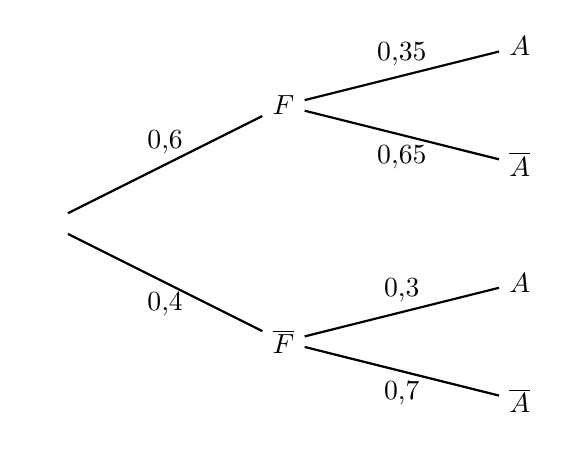
\begin{tikzpicture}[thick, scale=1.5]
\node (P_-1_0) at (-2,-1.5) {$\phantom{A}$};
\node (P_0_0) at (0,-0.5) {$F$};
\draw (P_-1_0) -- (P_0_0) node[midway, above] {$0{,}6$};
\node (P_1_0) at (2,-0) {$A$};
\draw (P_0_0) -- (P_1_0) node[midway, above] {$0{,}35$};
\node (P_1_1) at (2,-1) {$\overline{A}$};
\draw (P_0_0) -- (P_1_1) node[midway, below] {$0{,}65$};
\node (P_0_2) at (0,-2.5) {$\overline{F}$};
\draw (P_-1_0) -- (P_0_2) node[midway, below] {$0{,}4$};
\node (P_1_2) at (2,-2) {$A$};
\draw (P_0_2) -- (P_1_2) node[midway, above] {$0{,}3$};
\node (P_1_3) at (2,-3) {$\overline{A}$};
\draw (P_0_2) -- (P_1_3) node[midway, below] {$0{,}7$};
\end{tikzpicture}
\end{center}

\subsection*{2.}

\paragraph{a.} \(p(F \cap \overline{A}) = p(F) \times p_F(\overline{A}) = 0{,}6 \times 0{,}65 = 0{,}39\).

\paragraph{b.} 39 \% des campeurs viennent en famille mais ne profitent pas des activités du camping.

\subsection*{3.}

D'après la loi des probabilités totales :
\begin{align*}
p(A) &= p(F \cap A) + p(\overline{F} \cap A) \\
&= p(F) \times p_F(A) + p(\overline{F}) \times p_{\overline{F}}(A) \\
&= 0{,}6 \times 0{,}35 + 0{,}4 \times 0{,}3 \\
&= 0{,}21 + 0{,}12 = 0{,}33.
\end{align*}

\subsection*{4.}

Il faut trouver :
\[
p_{A}(F) = \dfrac{p(A \cap F)}{p(A)} = \dfrac{p(F \cap A)}{p(A)} = \dfrac{0{,}21}{0{,}33} = \dfrac{21}{33} = \dfrac{7}{11} \approx 0{,}636,
\]
soit \(0{,}64\) au centième près.

